\chapter{Implementation}\label{cha:implementation}

In this chapter, we discuss our author extraction implementation.
The following sections are structured similar to \Cref{cha:author-extraction}.
Thereby, we first look into the preprocessing steps.
We then consider the generation of distantly supervised training sets which includes creating a author knowledge, and the author name matching.
Using the reference strings with matched author names, we then build \gls{ge} constraints.
The last section of this chapter describes the learning of \glspl{linear-chain crf} using the reference strings as an unlabeled training set in combination with the generated \gls{ge} constraints.

The source code of the discussed implementation is available on GitHub\footnote{\url{https://github.com/mkrnr/reference-string-extraction} (accessed July~25,~2016)} under a GNU General Public License.

\section{Preprocessing}\label{sec:i-preprocessing}

The corpus that was used for our study consists of 32,470 research papers\footnote{The papers were downloaded on March~16,~2016.} that are accessible as \gls{pdf} documents via the \gls{ssoar}\footnote{\url{http://www.ssoar.info} (accessed April~21,~2016)}.
They are related to the area of social sciences\todo{stats on language}

Since our later steps require textual input, the first step is to extract the content from the \glspl{pdf}.
Apache PDFBox\footnote{\url{https://pdfbox.apache.org/} (accessed April~21,~2016)}, a Java library for manipulating \glspl{pdf}, allows the extraction of the content as Unicode text.
This is done by also taking into account the formatting of the document, for example when a research paper contain two text columns per page.
This way we were able to extract the text of 31,795 research papers.

\bigskip

After extracting the text from the \glspl{pdf}, the next step is to identify and extract reference sections.
As discussed in \Cref{sec:ae-preprocessing}, this is necessary to prevent the author matching algorithm from matching author names in the body of the research paper.

The reference string parsing package ParsCit\footnote{\url{http://wing.comp.nus.edu.sg/parsCit/} (accessed July~06,~2016)} uses regular expressions to identify the heading of a reference section by matching against strings such as ``References'', ``Bibliography'', or ``References and Notes''~\citep{councill2008parscit}.
Further heuristics detect whether a found reference section heading was found too early in the text~\citep{councill2008parscit}.
After the start is identified, another regular expression is used to search for the end of the reference section.

Yet, the implementation in ParsCit only considers research papers in the English language.
Thereby, German section headers such as ``Referenzen'' or ``Literaturverzeichnis'' are not covered by the regular expressions.
After adding a variety of German section headers to the ParsCit implementation, we encountered a high number of false positive matches.
In other words, many extracted reference sections did not contain reference strings.

As a result, we implemented our own approach which uses similar regular expressions and heuristics as the one of ParsCit.
Using this implementation, we were able to extract reference sections from 16,513 research papers.
A manual inspection showed a significantly smaller number of false positive in comparison to the extended ParsCit implementation.

\bigskip

Before using the extracted reference sections as an input for the author matching, we performed one further preprocessing step.
The reason for this is a reference style in which author names are separated by a slash instead of a space.
An example for this is the following reference string:
\begin{quote}
  Andretta, G./Baethge, M./Dittmer, S. 1994: Übergang wohin? Schwierigkeiten ostdeutscher Industriearbeiter bei ihrer betrieblichen Neuorientierung. In: SOFI-Mitteilungen Nr. 21/März 1994, Göttingen.
\end{quote}
Since we use whitespaces to separate words, without a preprocessing we would result in words such as ``G./Beathge,{}'' or ``M./Dittmer,{}''.
To prevent this, we add spaces around slashes.
For our example, this gives us:
\begin{quote}
  Andretta, G. / Baethge, M. / Dittmer, S. 1994: Übergang wohin? Schwierigkeiten ostdeutscher Industriearbeiter bei ihrer betrieblichen Neuorientierung. In: SOFI-Mitteilungen Nr. 21 / März 1994, Göttingen.
\end{quote}

\section{Generating Training Sets with Distant Supervision}\label{sec:i-distant-supervision}

\subsection{Knowledge Base Creation}\label{subsec:i-knowledge-base-creation}

In order to address \RQ{1} during our evaluation, we consider two different sources of author names.
Both have in common that author names are separated into first names and last names.

\bigskip

The first source is the \acrfull{gnd}\footnote{\url{http://www.dnb.de/EN/Standardisierung/GND/gnd.html} (accessed April~27,~2016)}\glsunset{gnd} -- German for integrated authority file --  which is published by the German National Library in cooperation with other library networks and institutions.
The \gls{gnd} contains information on persons, corporate bodies, conferences, and other topics with a focus on the German-speaking world which includes Germany, Austria, and Switzerland.
Further, it distinguishes between differentiated and undifferentiated person~\citep{hochstein2013ihr}.
A differentiated person is connected to exactly one individual whereas for an undifferentiated person, no such connection is modeled.
This for example is the case for historical personalities for which no precise records on their identity exist.

The \gls{gnd} data set is available under a Creative Commons Zero license and can be downloaded in the following formats: Marc 21, MARCXML, RDF/XML, Turtle, and JSON-LD.\@

For our author extraction, we use the Turtle format which is a format for \gls{rdf} data.
To extract the author names, we used the Apache Jena\footnote{\url{https://jena.apache.org/} (accessed July~25,~2016)} framework.
After loading the Turtle file into an \gls{rdf} triple store, we extracted the author names using a \gls{sparql} query.
The used \gls{sparql} query for extracting differentiated persons is shown in \Cref{fig:gnd-sparql-query}.
\lstset{language=SQL,morekeywords={PREFIX}}
\begin{figure}[t]
\begin{lstlisting}[basicstyle=\ttfamily]
PREFIX rdf: <http://www.w3.org/1999/02/22-rdf-syntax-ns#>
PREFIX gndo: <http://d-nb.info/standards/elementset/gnd#>
SELECT ?forename ?surname WHERE {
  ?person rdf:type gndo:DifferentiatedPerson .
  ?person gndo:preferredNameEntityForThePerson ?nameEntity .
  ?nameEntity gndo:forename ?forename .
  ?nameEntity gndo:surname ?surname .
}
\end{lstlisting}
\caption{\gls{sparql} query for extracting the preferred name of differentiated persons from the \gls{gnd} file given in a \gls{rdf} format.}
\label{fig:gnd-sparql-query}
\end{figure}
The \gls{gnd} file also contains name variations for some persons.
Yet, for our evaluation we only consider the name that is marked as ``preferred name''.

Due to the distinction between differentiated and undifferentiated names, we created two different lists of names.
One that only contains the names of differentiated persons and one that contains the names of both differentiated and undifferentiated persons.
We refer to the data sets as \texttt{gnd-diff} and \texttt{gnd-full}, respectively.
General statistics on the number of extracted names is shown in \Cref{tab:knowledge-base-statistics}.
The table also contains statistics on the number of individual names.

\begin{table}[t]
  \centering
\begin{tabular}{c c c c c c}
 \toprule
 & \texttt{gnd-full} & \texttt{gnd-diff} &\texttt{swp-trim} &\texttt{swp-full} & \begin{tabular}[c]{@{}c@{}}\texttt{swp-full}\\+\texttt{gnd-full}\end{tabular} \\
 \midrule
 \begin{tabular}[c]{@{}c@{}}Extracted\\Names\end{tabular} & 8,436,468 & 3,684,265 & 3,684,265& 10,796,240 & 19,232,708\\[5mm]
 \begin{tabular}[c]{@{}c@{}}Individual\\Names\end{tabular} &6,853,487 & 3,239,116 & 1,617,698 & 3,135,891 & 9,081,885\\
 %& & & & & \\
 \bottomrule
\end{tabular}
\caption{Statistics for different variations of the \texttt{gnd} and \texttt{swp} name lists.}
\label{tab:knowledge-base-statistics}
\end{table}

\bigskip

The second source is the social science portal Sowiport\footnote{\url{http://sowiport.gesis.org/} (accessed July~5,~2016)} which is maintained by GESIS --- Leibniz Institute for the Social Sciences.
From this portal, a list of author names was extracted via an Apache Solr\footnote{\url{http://lucene.apache.org/solr/} (accessed July~25,~2016)} query on June~13,~2016.
The results were provided in a \gls{xml} file.

In this file, an author name is represented as a string in which the last names are separated from the first names with a comma.
In some cases, multiple author names appear together in one string, separated by semicolons.

The Sowiport portal was chosen because of it's topical similarity to the research papers from the \gls{ssoar}.
We will refer to the second data set as the \texttt{swp} data set.
In order to allow a comparison to the \gls{gnd} data set, we additionally generated a version of the \texttt{swp} data set with the same number of authors as the \gls{gnd} data set.
We refer to this as the \texttt{swp-trim} data set.

\Cref{tab:knowledge-base-statistics}\todo{swp-full +gnd-full or +gnd-diff?} contains statistics on the different variations of the \texttt{gnd} and \texttt{swp} data sets.

\subsection{Author Name Matching}\label{subsec:i-author-name-matching}
Usually, matches are annotated using markup languages such as \gls{xml}.
For example, the third reference string in \Cref{fig:example-reference-strings} could be annotated with:
\begin{equation*}
  \texttt{<a><fn>}\text{Fritz}\texttt{</fn> <ln>}\text{M\"{u}ller,}\texttt{</ln></a> }\text{Fritz Schmidt (2010): \dots}
\end{equation*}
Here, \texttt{<a>\dots</a>} marks an author name, \texttt{<fn>\dots</fn>} a first name, and a last name is marked with \texttt{<ln>\dots</ln>}.
Since such markup language use tree based models, they do not allow a direct encoding of overlaps.
For example, assuming that we want to match all occurrences of the author ``Fritz M\"{u}ller'', the first three words of the previous example would need to be annotated with:
\begin{equation*}
  \texttt{<a><fn>}\text{Fritz}\texttt{</fn> <a><ln>}\text{M\"{u}ller,}\texttt{</ln></a> <fn>}\text{Fritz}\texttt{</fn></a>}
\end{equation*}
Yet, such a nesting of \gls{xml} tags is not allowed.
There are a number of approaches that try to overcome this limitation of tree based markup languages.
Examples are \textit{milestone elements}, \textit{fragmentation}, and \textit{standoff markup}~\citep{sperberg2000goddag}. They all drastically increase the complexity of the markup document and require specialized parsers in order to retrieve data from the documents.

To avoid this overhead, it would be preferable to annotate our author matches using a data structure that supports overlapping hierarchies by default.
\citet{sperberg2000goddag} propose such a data structure named \acrfull{goddag}\glsunset{goddag}.
Being a directed graph, it naturally solves the issue of overlaps by allowing a node to have multiple parents.
The graph has a hierarchy since it it acyclic.
In addition, it has ordered descendants.
Thereby, for any given node, the order of it's child nodes is defined.

\bigskip

Using the \gls{goddag} data structure, we will now discuss a concrete way of tagging author names in a given reference string.

As a first step, several variations of an author list described in \Cref{subsec:i-knowledge-base-creation} are generated.
For this, the author names are split into a set of first names and a set of last names.
If an author has multiple first names or last names, they are not further separated.
Thereby, we refer to them as \textit{full first names set} and \textit{full last names set}.
Since first names can be abbreviated in a reference, a next step is to generated a \textit{first name variations set}.
For example, given the full first name ``Max Friedrich'', we add the following variations to the first name variations set:
\begin{itemize}
  \itemsep0em
  \item Max
  \item Friedrich
  \item M.F
  \item MF
  \item M
  \item F
\end{itemize}
Note that no variation ends with a period.
This is because we later will ignore leading and trailing punctuation marks when matching names.

Further, we split entries in the full last names set that contain multiple last names, resulting in the \textit{single last names set}.

\bigskip

We now generate an initial \gls{goddag} structure for our given text.
This structure consists of a root node which has as child nodes the words of the reference section, separated at white space or new line characters.
These words are the leaf nodes of the \gls{goddag}.
The leaf nodes contain two representations of the word.
One that contains the word as it appears in the reference string, including it's leading and trailing non-word characters.
The other only contains the word itself, without leading and training non-word characters.
This allows an efficient name lookup in the following steps.

Given this initial \gls{goddag} structure, we now match the entries in the \textit{first name variations set} against the ``word'' properties of the leaf nodes.
If a match is found, a non-terminal node labeled ``FN'' is added between the root node and the matched leaf node.
In a second pass, we match against the \textit{single last names set} and add non-terminal nodes labeled ``LN'' accordingly.
We refer to the added nodes as \textit{first name nodes} and \textit{last name nodes}, respectively.

After the two iterations, a leaf node can simultaneously have a first name node and a last name node as its parent.
This again is not allowed in a tree-based structure such as \gls{xml}.

\Cref{fig:example-goddag-4-names} shows a \gls{goddag} for the fourth reference string in \Cref{fig:example-reference-strings} with matched first names and last names.
Here, The word ``Friedrich'' is tagged as both a possible first name and last name.
Note that in our evaluation, we use one \gls{goddag} per reference section.
\begin{figure}[t]
  \centering
%\hspace*{-1.25cm}
\resizebox{\linewidth}{!}{%
  % Mia Wagner, Max Friedrich Schmidt (2010): Fourth title, Berlin: Springer.
\begin{tikzpicture}
  \tikzset{ellipsenode/.style={ellipse,thick,draw}}
\tikzset{rectanglenode/.style={rectangle,draw}}
\tikzset{directededge/.style={->,> = latex,thick}}



  \node[rectanglenode] (l1)                       {\vp Mia};
  \node[rectanglenode] (l2)  [right=of l1]        {\vp Wagner,};
  \node[rectanglenode] (l3)  [right=of l2]        {\vp Max};
  \node[rectanglenode] (l4)  [right=of l3]        {\vp Friedrich};
  \node[rectanglenode] (l5)  [right=of l4]        {\vp Schmidt};
  \node                (l6)  [right=0.3cm of l5]  {\vp\textbf{\dots}};
  \node[rectanglenode] (l7)  [right=0.25cm of l6] {\vp Springer.};
  \node[ellipsenode]   (fn1) [above=of l1]        {FN};
  \node[ellipsenode]   (ln1) [above=of l2]        {LN};
  \node[ellipsenode]   (fn2) [above=of l3]        {FN};
  \node[ellipsenode]   (ln2) [right=0.5cm of fn2] {LN};
  \node[ellipsenode]   (fn3) [right=0.5cm of ln2] {FN};
  \node[ellipsenode]   (ln3) [above=of l5]        {LN};
  \node[ellipsenode]   (o1)  [above=of l7]        {O};
  \node[ellipsenode]   (r)   [above=of ln2]       {root};

  \foreach \from/\to in {r/fn1,r/ln1,r/fn2,r/ln2,r/fn3,r/ln3,r/o1,fn1/l1,ln1/l2,fn2/l3,ln2/l4,fn3/l4,ln3/l5,o1/l7}
  \draw[directededge] (\from) -- (\to);
\end{tikzpicture}


}
\caption{\gls{goddag} for the fourth reference string in \Cref{fig:example-reference-strings} with matched first names and last names from \Cref{tab:example-author-list}.}
\label{fig:example-goddag-4-names}
\end{figure}

\bigskip

The goal now is to match the list of authors against the \gls{goddag} structure with identified first names and last names.
For this, we generate an \textit{author name map} that contains as keys the entries from the full last names set.
As values, it contains the first name variations of first names that appear together with the given last names in our original author list.

Given this map, we iterate over the leaf nodes using a sliding window approach.
First, we examine if one or more neighboring leaf nodes have a last name parent node.
If this is the case, we examine their neighboring leaf nodes for first name parent nodes.
If both last name parent nodes and neighboring first name parent nodes are found, a lookup in the author name map is performed using the ``word'' property of the leaf nodes.

If a match is found, a non-terminal node with the label ``AU'' for author is inserted between the root node and the corresponding parents of the matched leaf nodes.

\Cref{fig:example-goddag-4-final} shows a \gls{goddag} for the fourth reference string in \Cref{fig:example-reference-strings} that includes three matches from the author list in \Cref{tab:example-author-list}.
\begin{figure}[t]
  \centering
\resizebox{\linewidth}{!}{%
  % Mia Wagner, Max Friedrich Schmidt (2010): Fourth title, Berlin: Springer.
\begin{tikzpicture}
  \tikzset{ellipsenode/.style={ellipse,thick,draw}}
\tikzset{rectanglenode/.style={rectangle,draw}}
\tikzset{directededge/.style={->,> = latex,thick}}



  \node[rectanglenode] (l1)                       {\vp Mia};
  \node[rectanglenode] (l2)  [right=of l1]        {\vp Wagner,};
  \node[rectanglenode] (l3)  [right=of l2]        {\vp Max};
  \node[rectanglenode] (l4)  [right=of l3]        {\vp Friedrich};
  \node[rectanglenode] (l5)  [right=of l4]        {\vp Schmidt};
  \node                (l6)  [right=0.3cm of l5]  {\vp \textbf{\dots}};
  \node[rectanglenode] (l7)  [right=0.25cm of l6] {\vp Springer.};
  \node[ellipsenode]   (fn1) [above=of l1]        {FN};
  \node[ellipsenode]   (ln1) [above=of l2]        {LN};
  \node[ellipsenode]   (fn2) [above=of l3]        {FN};
  \node[ellipsenode]   (ln2) [right=0.5cm of fn2] {LN};
  \node[ellipsenode]   (fn3) [right=0.5cm of ln2] {FN};
  \node[ellipsenode]   (ln3) [above=of l5]        {LN};
  \node[ellipsenode]   (o1)  [above=of l7]        {O};
  \node[ellipsenode]   (a1)  [above right=of fn1] {AU};
  \node[ellipsenode]   (a2)  [right=of a1]        {AU};
  \node[ellipsenode]   (a3)  [right=of a2]        {AU};
  \node[ellipsenode]   (r)   [above right=of a1]  {root};

  \foreach \from/\to in {r/a1,r/a2,r/a3,r/o1,a1/fn1,a1/ln1,a2/fn2,a2/ln2,a3/fn2,a3/fn3,a3/ln3,fn1/l1,ln1/l2,fn2/l3,ln2/l4,fn3/l4,ln3/l5,o1/l7}
  \draw[directededge] (\from) -- (\to);
\end{tikzpicture}


}
\caption{Final \gls{goddag} for the fourth reference string in \Cref{fig:example-reference-strings}.}
\label{fig:example-goddag-4-final}
\end{figure}
In \Cref{app:author-name-matching}, we present the \glspl{goddag} for the three remaining reference strings of \Cref{fig:example-reference-strings}.

\section{Building \glsentryshort{ge} Constraints}\label{sec:i-building-ge-constraints}

We now use the created \gls{goddag} structures with matched author names to create \gls{ge} constraints.
To recall from \Cref{sec:ae-building-ge-constraints}, a \gls{ge} constraint is a \gls{probability distribution} $\tilde{P}(Y_n)$ for a word $w_n$ in the reference section where $\textit{Val}(Y_n)$ is the set of possible labels for this word:
\begin{equation*}
  \mathit{Val}(Y_n)=\{\texttt{B-FN},\texttt{B-LN},\texttt{I-FN},\texttt{I-LN},\texttt{O}\}
\end{equation*}
We can derive this \gls{probability distribution} from the \glspl{goddag} by iterating over the children of the root node and.
When reaching an author node, we can add the according probability mass to the probability distributions of of it's children.

For example, the first author node in \Cref{fig:example-goddag-4-final} contains a first name node and a last name node.
Since the children are ordered, the first name node appears first in the sequence.
Thereby, we add a probability mass of one to the label \texttt{B-FN} of the word ``Mia'' and to the label \texttt{I-LN} of the word ``Wagner,''.
This shows the importance of having ordered children in this graph structure.

\Cref{tab:example-ge-constraints} shows the resulting \gls{ge} constraints for the four \glspl{goddag} that were derived from the matched of the author list in \Cref{tab:example-author-list} with the reference strings in \Cref{fig:example-reference-strings}.
As we discussed in \Cref{sec:ae-building-ge-constraints}, for this example we also include every third word that is not matched to an author name, starting with ``(2010):'' in the first reference string.

\section{Learning \glsentryshortpl{crf}}\label{sec:i-learning-crfs}

After presenting our approach on generating \gls{ge} constraints, we now discuss the implementation for the learning of \glspl{linear-chain crf} which uses an unlabeled set of reference sections and the corresponding \gls{ge} constraints as an input.

We use the \acrfull{mallet}\glsunset{mallet}~\citep{mccallum2002mallet} for most of the implementation discussed in this section.
\gls{mallet} is an open-source Java library that includes tools for tasks such as document classification, sequence tagging, or topic modeling.
Especially relevant for us is its implementation of \glspl{linear-chain crf} since it can be learned using a list of \gls{ge} constraints.
The learning is performed using gradient ascent with a limited memory \gls{bfgs} approximation (see \Cref{sec:learning-crfs}).

\subsection{Graph Construction}\label{subsec:i-graph-construction}

Based on the discussion in \Cref{subsec:ae-graph-construction}, we focus on the construction of \glspl{linear-chain crf}.

In \gls{mallet}, it is possible to create \glspl{linear-chain crf} with different Markov orders (see \Cref{subsec:ae-graph-construction}).
More specifically, the Markov order is declared using an integer array with non-negative numbers in increasing order.
The highest integer specifies the Markov order of the \gls{crf}.
The other numbers represent additional weight sets to also model lower Markov orders in the same model.
% from MALLET documentation:
% * @param orders an array of increasing non-negative numbers giving
% * the orders of the features for this CRF. The largest number
% * <em>n</em> is the Markov order of the CRF. States are
% * <em>n</em>-tuples of output labels. Each of the other numbers
% * <em>k</em> in <code>orders</code> represents a weight set shared
% * by all destination states whose last (most recent) <em>k</em>
% * labels agree. If <code>orders</code> is <code>null</code>, an
% * order-0 CRF is built.

For example, an integer array \texttt{[0,1]} specifies an Markov order $1$ \gls{linear-chain crf} and an additional weight set for the Markov order $0$ states.
When modeled with \glspl{factor}, the Markov order $0$ state for a word $w_n$ only includes the \gls{target variable} $Y_n$: $\Psi(Y_n)$.
Applied to the author extraction example from \Cref{cha:crfs}, this specification results in a \gls{factor graph} shown in \Cref{fig:example-linear-chain-crf-markov-order-0-1}.
\begin{figure}[t]
\centering
\newcommand{\factorgraphnodes}{%
  \node[latent] (start) {\texttt{start}}; %
  \node[latent, right=2.4cm of start] (ln) {$LN_1$}; %
  \node[latent, right=2.4cm of ln] (fn) {$F\rs N_2$}; %
  \node[obs, below=1.8cm of ln] (ec1) {$EC_1$}; %
  \node[obs, below=1.8cm of fn] (ec2) {$EC_2$}; %
}
\begin{tikzpicture}
  \factorgraphnodes

  \factor[right=1.1cm of start] {start-ln-f} {above:$\Psi(\texttt{start},LN_1)$} {} {}; %
  \factor[right=1.1cm of ln] {ln-fn-f} {above:$\Psi(LN_1,F\rs N_2)$} {} {}; %
  \factor[above=0.8cm of ec1] {ec1-ln-f} {left:$\Psi(LN_1,EC_1)$} {} {}; %
  \factor[above=0.8cm of ec2] {ec2-fn-f} {left:$\Psi(F\rs N_2,EC_2)$} {} {}; %
  \factor[above=0.8cm of ln] {ln-f} {left:$\Psi(LN_1)$} {} {}; %
  \factor[above=0.8cm of fn] {fn-f} {left:$\Psi(F\rs N_2)$} {} {}; %
  \edge[-] {start} {ln};
  \edge[-] {ln} {fn};
  \edge[-] {ln} {ec1};
  \edge[-] {fn} {ec2};
  \edge[-] {ln} {ln-f};
  \edge[-] {fn} {fn-f};
\end{tikzpicture}

\caption{%
  \Gls{factor graph} of a \gls{linear-chain crf} with both Markov order $0$ and $1$, derived from the author extraction example in \Cref{cha:crfs}.}
\label{fig:example-linear-chain-crf-markov-order-0-1}
\end{figure}

\subsection{Model Parameters}\label{subsec:i-model-parameters}

The implementation of \glspl{linear-chain crf} in \gls{mallet} allows the modification of several model parameters.
One that is addressed by \RQ{8} is the regularization parameter of the Gaussian prior (see \Cref{sec:learning-crfs}).
The default for this parameter is set to $10$.

Further, we can specify the maximum number of iterations during the learning with gradient ascent.
In our evaluation setup, it was sufficient to set this number to a high value, in our case $10,000$ since the learning always converged in a reasonable time.

A last parameter that we can specify is the number of resets of the L-\gls{bfgs} calculation.
This can improve the result of the learning since the \dots\todo{continue based on distant supervision section}
Yet, empirical tests have shown that for our evaluation, modifying this parameter does not have a significant impact on the resulting model.
Thereby, we set the number of resets to $4$ for all experiments.

\subsection{Feature Engineering}\label{subsec:i-feature-engineering}

To create features in \gls{mallet}, they are added via so-called \textit{pipes}.
A first step is to transform a given input string into a vector of \textit{tokens}.
In our case, the input string is a reference section and a token contains a word in the reference string, separated by whitespaces.

It is now possible to assign different features to the tokens.
The local features that we use for the evaluation (see \Cref{tab:our-features-regular-expressions}), are implemented using a variation of the \texttt{cc.mallet.pipe.tsf.RegexMatches} class.
This class matches words against a regular expression that describes a feature.
If a match was found, it assigns a feature label with an initial weight of $1$.
The Java regular expressions that we use for detecting different local features are shown in \Cref{app:sec-feature-engineering}.

Further, we consider two lexicon features, FIRSTNAME and LASTNAME\@.
We use the two of the lists that we created for the author name matching in \Cref{subsec:i-author-name-matching} as lexica.
Tokens are assigned the feature label FIRSTNAME if the contained word appears in the first name variations set.
Consequently, the feature label LASTNAME is assigned if the word appears in the single last name set.
In our evaluation, the feature weight is the natural logarithm of the frequency of the word in the original author name knowledge base.
For example, in the \texttt{swp} data set, the first name ``Max'' was part of $11,618$ author names.
Thereby, we assign the feature weight $\ln(11,618)\approx9.3603$ to a token that contains the first name ``Max''.

